\documentclass{bakalarka}
%\usepackage[cp1250]{inputenc}
\usepackage[utf8]{inputenc} 
\usepackage[czech]{babel}
\usepackage{ae}
\usepackage{fancyhdr}
\usepackage{float}
\usepackage{graphicx}
%\usepackage[pdftex]{graphicx}
\author{Martin Kadlec}
\title{Docháka a výkazy práce pro systém IMIS na platformě Android}
\titlet{}
\titlett{}
\university{Západočeská univerzita v Plzni}
\faculty{Fakulta aplikovaných věd}
\department{Katedra informatiky a výpočetní techniky}
\subject{Diplomová práce}
\town{Plzeň}
\begin{document}
\pagestyle{fancy}
\renewcommand{\chaptermark}[1]{\markboth{\textit{#1}}{}}
\renewcommand{\sectionmark}[1]{\markright{\textit{#1}}{}}
\cfoot{\thepage}
\lhead{\leftmark}
\rhead{\rightmark}
\maketitle
\chapter*{Prohlížení}
\thispagestyle{empty}
Prohlašuji, že jsem bakalářskou práci vypracoval samostatně a výhradně s~použitím citovaných pramenů.
\vskip 1.5em
V Plzni dne \today
\vskip 0.7em
\hskip 9cm Maxipes Fík
\chapter*{Abstract}
\thispagestyle{empty}
Text of abstract.
\tableofcontents
\pagestyle{fancy}
\renewcommand{\chaptermark}[1]{\markboth{\textit{#1}}{}}
\renewcommand{\sectionmark}[1]{\markright{\textit{#1}}{}}
\cfoot{\thepage}
\lhead{\leftmark}
\rhead{\rightmark}
\parskip 1em
\chapter{Úvod}

\section{Zásady pro vypracování}
\begin{enumerate}
\item Prozkoumejte systém IMIS pro evidenci docházky a pracovních výkazů. Vyberte činnosti, které by bylo vhodné implementovat i pro mobilní zařízení.
\item Navrhněte mobilní aplikaci pro platformu Android, které bude obsahovat vybrané funkce z předchozího bodu zadání.
Zvažte aspekty zabezpečení komunikace aplikace se systémem.
\item Implementujte navržené řešení, berte přitom v úvahu možnou rozšiřitelnost o další funkce.
\item Ověřte funkcionalitu vytvořené aplikace.
\end{enumerate}



\section{Současný systém}
IMIS = Integrovaný manažerský informační systém\\

Oracle Forms 6i - tlustý klient \\
\begin{verbatim}
http://en.wikipedia.org/wiki/Oracle_Forms
\end{verbatim}

- moduly:\\
Object Library\\
PL/SQL Library  \\
Form Module   \\
Menu Module\\
- bloky:\\
Data blocks\\
Control blocks\\

- ukazky implementovanych formularu, GUI-popis\\
- datovy model\\

\section{Oracle forms}

\paragraph{PL/SQL}
PL/SQL (Procedural Language/Structured Query Language) je procedurální nadstavba jazyka SQL od firmy Oracle založená na programovacím jazyku Ada.
\begin{figure}[H]
  \centering
  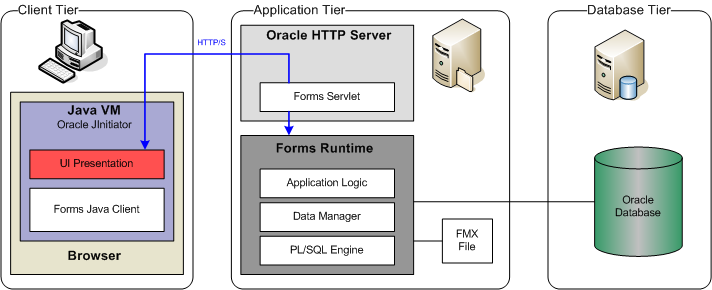
\includegraphics[scale=0.55]{obr/3tier.png}
  \label{}
\end{figure}
TODO zobrazit jako desktop klienta
\section{Datový model}

\section{Forms klient}

\subsection{Zápis příchodů a odchodů}
\begin{figure}[H]
  \centering
  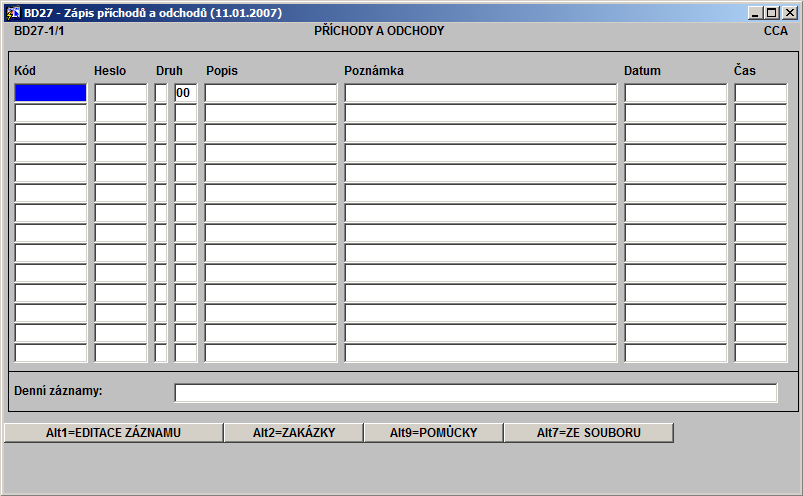
\includegraphics[scale=0.6]{obr/BD27.png}
  \label{}
\end{figure}

\subsection{Výkaz práce}
\begin{figure}[H]
  \centering
  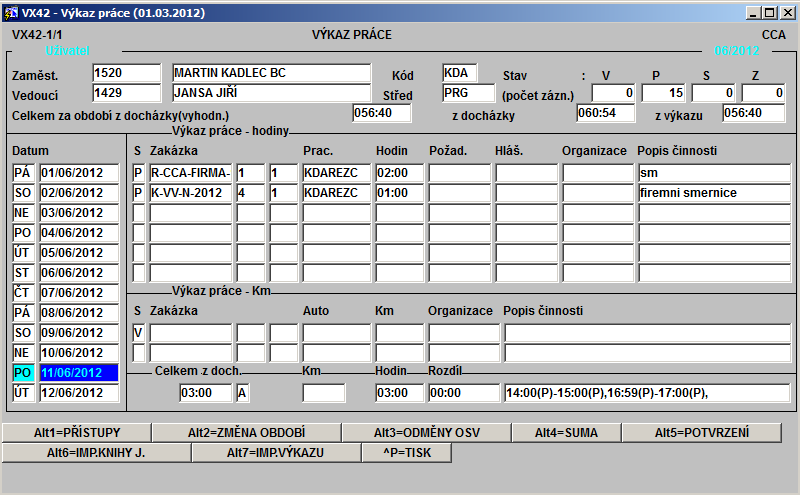
\includegraphics[scale=0.6]{obr/VX42.png}
  \label{}
\end{figure}

\section{Triggery}
jen ty, jejichž funkčnost bude muset být implementována.

\chapter{Implementace}

\section{Funkcionalita}

\section{Výběr achitektury}
vhodne prostredky: JDBC/webova sluzby/Oracle Database Mobile Server 11g - zajistuje synchronizaci mezi Oracle db a mobilnim zarizenim, zamitnuto z licencnich duvodu, mozna by stalo za to to vic prozkoumat a neco o tom napsat
\section{Architektura}
Android aplikace funguje jako tenký klient, který se připojuje k webové službě. Webová služba používá REST architekturu a přistupuje k samotné databázi.

\begin{figure}[H]
  \centering
  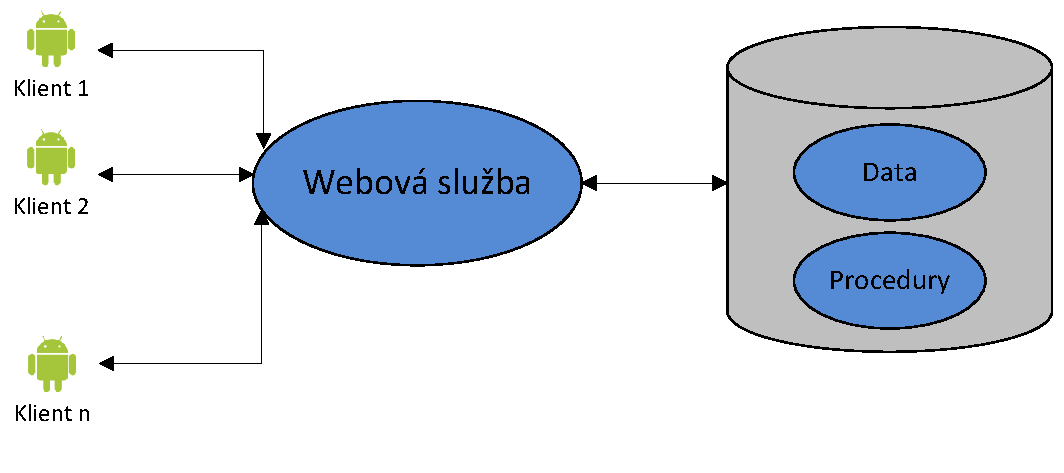
\includegraphics[scale=0.8]{obr/souc_arch2.pdf}
  \label{obr: logo zcu}
\end{figure}

\begin{itemize}
\item Webová služba - Java EE 6, aplikační server GlassFish
\item Databáze - Oracle 10g, obsahuje navíc databázové procedury, které se používají v současných formulářích  
\item Android - obsahuje persistentní úložiště, obsahuje záznamy o docházce (tabulka KARTA - v datovém modelu), úložiště se bude automaticky synchronizovat ve stavu online s databázovým serverem prostřednictvím webové služby
\end{itemize}

V knihovnách pro Forms aplikace se nachází další kód, který bude nutné přepsat do webové služby.
\section{REST}
\begin{enumerate}
\item REST operace - davkove vs jednotlive
\item REST, tabulka URI, 
\end{enumerate}

\section{Synchronizace}
\begin{enumerate}
\item sync algoritmus - 2 algoritmy (jeden ideální, druhý reálný), srovnání
\item sync architektura - komponenty
\end{enumerate}

\section{Zabezpečení}
Server webové služby je dostupná v síti VPN. Další zabezpečení bude řešeno později...

\section{O čem psát...}
\begin{enumerate}
\item vyuziti soucasneho kodu z knihoven - databazove baliky a PLL forms knihovny
\item datovy model, na strane androida jen jeho podmnozina, napr ciselniky..
\item popsat IMIS 
\item ROWID jako unikatni identifikator, problemy ktere to prinasi
\item pripraveno webove sluzby na dalsi mobilni platformy
\item cinnost apliakce online/offline
\item flow diagramy pro ruzne cinnosti
\item pristupova prava
\item uspora pesistentni pameti na strane androida
\item chybove reporty a opravy na aplikaci v ostrem prostredi
\item jak zjisit zmenu zaznamu, v datech se uklada pouze datum posledni zmeny, nikoli presny cas
\item výhrady v db schématu
\item android komponenty pro sync, authentikaci..., nestandartni UI atd...
\end{enumerate}

\appendix
\bibliographystyle{csplainnat}
%\bibliography{bakalarka}
\end{document}
